% ===========================================================================
%  EUROGRAPHICS 2027 -- full paper (proceedings in Computer Graphics Forum)
%  Working title: Sequential Score Pre-computation for Video Diffusion
%
%  BUILD REQUIREMENTS
%  ------------------
%  This draft uses a GENERIC, stock class (article, two-column) so it compiles
%  anywhere with no external kit:
%
%      pdflatex main ; bibtex main ; pdflatex main ; pdflatex main
%
%  TO SWAP IN THE EUROGRAPHICS/CGF KIT at submission time:
%    1. Replace the \documentclass line below with   \documentclass{egpubDL}
%    2. Replace the generic author block (\author{...}) with the EG block kept
%       verbatim in the "EG AUTHOR BLOCK" comment beside it.
%    3. Uncomment the \teaser{...} block and the \begin{classification} CCS block.
%    4. Set \bibliographystyle{eg-alpha-doi} (see the bibliography line).
%  egpubDL.cls and eg-alpha-doi.bst ship in the EG author kit and are NOT
%  vendored here (not redistributable). Every EG-only construct is tagged
%  "% EG-KIT:" so the swap is a grep.
%
%  STATUS LEGEND used throughout:
%     [WRITTEN]  -- content backed by a measured result in this repo.
%     TODO(...)  -- a placeholder that MUST be filled before submission.
%
%  CLAIM DISCIPLINE (do not relax): every speedup is FITTING/PRECOMPUTE
%  wall-clock, never sampling; every quality comparison must be at matched
%  wall-clock; nothing may imply volumetric/4D support -- the domain is
%  2D dynamic video (T x H x W).
% ===========================================================================

\documentclass[10pt,twocolumn]{article}      % EG-KIT: replace with \documentclass{egpubDL}

\usepackage[a4paper,margin=1.8cm]{geometry}  % EG-KIT: delete (class sets the layout)
\usepackage[T1]{fontenc}
\usepackage{amsmath}
\usepackage{amssymb}
\usepackage{amsthm}
\usepackage{graphicx}
\usepackage{booktabs}
\usepackage{multirow}
\usepackage{subcaption}
\usepackage{algorithm}
\usepackage{algpseudocode}
\usepackage{url}
\usepackage{xcolor}
\graphicspath{{./figures/}}

% Lightweight editorial marker for the drafting phase. Delete before submission.
\newcommand{\todo}[1]{{\color{red}\textbf{[TODO: #1]}}}
\newcommand{\needsnum}[1]{{\color{red}\underline{#1}}} % a number awaiting a run

\theoremstyle{plain}
\newtheorem{proposition}{Proposition}
\newtheorem{remark}{Remark}

% ---------------------------------------------------------------------------
\begin{document}

% --- Generic title/author block (compiles under article). ---
% EG-KIT: replace this whole block with the "EG AUTHOR BLOCK" below it.
\title{Sequential Score Pre-computation for Video Diffusion via\\
       Upwind Fokker--Planck Solves, KL-Triggered Keyframing,\\
       and Krylov-Projected Physical Control}
\author{%
  A.\,S.~Na\thanks{Corresponding author: andrew.na@uwaterloo.ca} \and
  W.~Gao \and M.~Briazkalo \and J.\,W.\,L.~Wan\\
  \normalsize David R. Cheriton School of Computer Science,
  University of Waterloo, Ontario, Canada}
\date{}

% EG AUTHOR BLOCK (kit convention: running-head list in [], full block in {}).
% EG-KIT: uncomment the following and delete the generic block above.
% \title[Sequential Score Pre-computation for Video Diffusion]%
%       {Sequential Score Pre-computation for Video Diffusion via\\
%        Upwind Fokker--Planck Solves, KL-Triggered Keyframing,\\
%        and Krylov-Projected Physical Control}
% \author[A.\,S.~Na, W.~Gao, M.~Briazkalo \& J.\,W.\,L.~Wan]{%
%   \parbox{\textwidth}{\centering
%     A.\,S.~Na\textsuperscript{1}\thanks{Corresponding author: andrew.na@uwaterloo.ca}
%     \quad W.~Gao\textsuperscript{1}
%     \quad M.~Briazkalo\textsuperscript{1}
%     \quad J.\,W.\,L.~Wan\textsuperscript{1}}
%   \\
%   {\parbox{\textwidth}{\centering
%     \textsuperscript{1}David R. Cheriton School of Computer Science,
%     University of Waterloo, Ontario, Canada}}
% }

% -- Teaser: object-removal before/after strip. Asset not yet rendered.
% EG-KIT: \teaser is provided by egpubDL; uncomment at submission.
% \teaser{
%   \includegraphics[width=\linewidth]{teaser_object_removal}
%   \centering
%   \caption{TODO(teaser): input clip, mask, and our temporally-coherent fill,
%            side by side across frames. Render from run_video.py on a DAVIS clip.}
%   \label{fig:teaser}
% }

\maketitle

% ===========================================================================
\begin{abstract}
Training-free, per-instance diffusion priors are attractive for video editing
because they require no external training corpus, but fitting them is dominated
by the cost of estimating the score field. We extend a per-instance score
\emph{pre-computation} scheme -- in which the log-density Fokker--Planck (FP)
equation is solved numerically \emph{before} network fitting rather than being
learned -- from single images to \textbf{2D dynamic video} ($T\times H\times W$:
two spatial dimensions plus time). Our contributions are numerical and
systems-level. First, we discretise the video FP operator with an
\emph{upwind} stencil and solve it by line Gauss--Seidel relaxation; the
resulting operator is an M-matrix with a row-dominance margin of exactly one for
every configuration we tested, which removes the $\sigma^2\Delta t\le\tfrac12$
stability restriction of the central-difference scheme entirely. We report the
cost of that guarantee honestly: the scheme is first-order and injects
artificial diffusion of $|s|h/2$. Second, exploiting the near-identity of the FP
operator between consecutive frames, we perform \emph{sequential importance
sampling} on the low-dimensional density-estimation coordinates and trigger a
full re-estimate only when a Kullback--Leibler statistic on the importance
weights indicates the warped proposal has failed; this incremental correction is
$7.5\times$ cheaper per frame than re-estimation while detecting scene cuts with
zero false positives on our control sequence. Third, we guide the inpainting
itself with \emph{physical control}: linear constraints---temporal
flow-consistency foremost---are enforced by projecting the sampler state onto
the constraint manifold at every integration step, solved matrix-free by a
warm-started Krylov (conjugate-gradient) iteration on the normal equations, with
adjoints obtained exactly by automatic differentiation. We instantiate the pipeline for
per-instance video inpainting / object removal, where fitting to a single clip
is the accepted methodology and temporal incoherence is the metric of interest.
\emph{All speedups are fitting/pre-compute wall-clock, not sampling.}
\end{abstract}

% EG-KIT: the ACM CCS classification block below is rendered by egpubDL inside
% the abstract. Uncomment it there and delete this \keywords line at submission.
\medskip\noindent\textbf{CCS Concepts / Keywords:}
video diffusion; per-instance fitting; Fokker--Planck; upwind finite differences;
M-matrix stability; sequential importance sampling; constrained sampling;
Krylov projection; video inpainting.
% \begin{classification} % https://www.acm.org/publications/class-2012
% \CCScat{Computing methodologies}{Computer graphics}{Image manipulation}{Computational photography}
% \CCScat{Mathematics of computing}{Numerical analysis}{Partial differential equations}{}
% \end{classification}

% ===========================================================================
\section{Introduction}
% [WRITTEN -- framing is fixed and defensible]

Diffusion models are now the dominant tool for image and video synthesis, but a
diffusion \emph{prior} is expensive to obtain: it is normally amortised by
training a network on a large corpus. A complementary line of work fits a prior
to a \emph{single} instance -- one image, or here one clip -- with no external
training data. This per-instance regime, in the lineage of the Deep Image
Prior~\cite{ulyanov-2018-dip}, is exactly the setting where video editing tasks
such as inpainting and object removal are most naturally posed: the content to
be respected is the clip in front of you, not a dataset.

This paper builds on a per-instance \emph{score pre-computation} scheme for
score-based diffusion~\cite{ysong-2020}. Rather than learning the score
$\nabla_x\log p$ with a network, the log-density FP equation is solved
numerically before fitting, and the pre-computed score is embedded into the
training signal. On single images this reduces fitting wall-clock
substantially. We extend it to video and confront the two problems that
appear the moment a temporal axis is added: (i) the numerical stability of the
FP solve on a three-axis grid, and (ii) the cost of re-estimating the density
for every frame when consecutive frames are nearly identical.

\medskip\noindent\textbf{Scope: 2D dynamic video.} The domain is
$T\times H\times W$ throughout. The FP solve runs on a three-axis grid, but two
of those axes are pixel-\emph{value} axes and the third is time; this is 2D
imagery in motion, not volumetric or 4D data. Dynamic 3D/4D representations
(deformable Gaussians, dynamic NeRF) are out of scope. Where the implementation
says ``3D operator'' it refers to the three axes of the linear system.

\medskip\noindent\textbf{Regime and claim discipline.} This is a per-instance
pre-computation and fitting accelerator, \emph{not} a generative model of a data
distribution. Reported quality is measured against the fitted clip, and every
speedup is \emph{fitting/pre-compute} wall-clock, never sampling. We state this
in the abstract, here, and in every table caption, because the distinction is
easy to lose.

\medskip\noindent\textbf{Contributions.} The pipeline is made practical by two
mechanisms---\emph{importance sampling} for speed and a \emph{Krylov projection}
for control---on the numerical foundation of a stable FP solver:
\begin{enumerate}
  \item An \textbf{unconditionally stable} video FP solver: an upwind
        discretisation solved by full-diagonal line Gauss--Seidel, proven an
        M-matrix in practice (dominance margin exactly $1.0$ across all tested
        $\sigma$, $N$, $|s|$), matching the unsplit solve to $4.6\times10^{-9}$.
        We quantify its first-order accuracy cost exactly (Sec.~\ref{sec:stab}).
  \item \textbf{Speed --- a KL-triggered sequential importance sampler} that
        accelerates the KDE-based score solve: it reuses the
        previous frame's converged density as a motion-warped proposal and
        re-estimates only on demand, $7.5\times$ cheaper per frame than
        per-frame re-estimation, with a keyframe rule that is interpretable as a
        scene-cut / disocclusion detector (Sec.~\ref{sec:keyframe}).
  \item \textbf{Control --- a Krylov-projected constraint framework} that guides
        the inpainting: physical linear constraints $Cx=d$ (temporal
        flow-consistency foremost) are imposed by projecting the sampler state
        onto the constraint manifold each step, solved matrix-free by
        conjugate gradients on the SPD normal equations with automatic-
        differentiation adjoints and warm starts across steps. We validate the
        projection numerically and measure its effect on quality: enabling
        flow-consistency control cuts masked warping error by $50.5\%$ across
        $70$ DAVIS clips and three seeds (Sec.~\ref{sec:control-results}).
  \item A per-instance \textbf{video inpainting} instantiation with masked,
        motion-compensated evaluation, and an honest account of where the
        temporal path does and does not yet help (Sec.~\ref{sec:exp}).
\end{enumerate}

% ===========================================================================
\section{Related Work}
% [WRITTEN -- structure fixed; expand prose and complete citations]

\noindent\textbf{Score-based and denoising diffusion.} SMLD~\cite{ysong-2019},
DDPM~\cite{ho-2020} and the unifying SDE
framework~\cite{ysong-2020,sohl-dickstein-2015} parameterise data corruption as
a stochastic process and learn the score by denoising score
matching~\cite{hyvarinen-2005,vincent-2011}.

\noindent\textbf{Fast sampling.} DDIM~\cite{jsong-2020} and dedicated ODE
solvers, DPM-Solver / DPM-Solver++~\cite{lu-2022,lu-2022-dpmpp}, and distilled
or few-step models -- consistency models~\cite{song-2023-consistency}, rectified
flow~\cite{liu-2023-rectified} -- attack \emph{sampling} cost. Our contribution
is orthogonal: it reduces \emph{fitting} cost. \todo{make the orthogonality
explicit and cite the one-sentence distinction reviewers will look for.}

\noindent\textbf{FP equation and diffusion.} The connection between the forward
SDE, reverse SDE and FP equation is classical~\cite{anderson-1982,oksendal-1987}.
FP-Diffusion~\cite{lai-2022} adds a score-FP regulariser under regularity
conditions; Boffi and Vanden-Eijnden~\cite{boffi-2022} solve the probability-flow
equation with networks. We instead solve the log-density FP equation directly by
finite differences, avoiding both the network-per-timestep cost and the
regularity assumptions.

\noindent\textbf{Video diffusion.} Trained video diffusion
models~\cite{ho-2022-video,blattmann-2023-svd} are a different setting (large
corpora, sampling-time cost) and are reported as clearly-labelled context, not as
matched baselines. \todo{add 1--2 recent (2024--2026) video inpainting / object
removal methods; identify at least one zero-shot / internal-learning method as a
same-category comparison~\cite{ouyang-2021-internal}.}

\noindent\textbf{Numerics.} Upwinding, M-matrices and the discrete maximum
principle are standard~\cite{leveque-2007,morton-mayers-2005,varga-2000}; line
relaxation and ADI descend from~\cite{peaceman-rachford-1955}. Sequential
importance sampling and effective sample size come from the SMC
literature~\cite{doucet-2001-smc,kong-1994-ess}. Krylov subspace methods and
warm-started conjugate gradients on the normal equations are
classical~\cite{saad-2003-iterative,hestenes-1952-cg}. Motion fields use
RAFT~\cite{teed-2020-raft}.

\noindent\textbf{Constrained and guided sampling.} A parallel line conditions
diffusion samplers on measurements or physical priors---replacement/projection
inpainting~\cite{lugmayr-2022-repaint}, diffusion posterior
sampling and its manifold-constrained variants~\cite{chung-2023-dps}. We differ
by treating the guidance as an \emph{explicit linear projection} onto $\{Cx=d\}$
solved matrix-free by a Krylov iteration, rather than a score-space gradient,
which makes the known-region constraint exact and composes arbitrary physical
constraints without retraining. The per-step correction is a minimum-effort
control whose KKT/saddle system and its Tikhonov-regularised reduction are
standard in PDE-constrained optimisation and equality-constrained least
squares~\cite{nocedal-2006-numopt,benzi-2005-saddle}. \todo{cite: verify RePaint,
DPS/MCG, and one optical-flow-consistent video editing/inpainting method as the
closest prior.}

% ===========================================================================
\section{Background: score pre-computation}
% [WRITTEN -- carried and condensed from the image paper]

For $t\in[0,T]$ a clip frame $x(t)\in\mathbb{R}^{H\times W}$ evolves under a
forward SDE
\begin{equation}
  dx(t) = f(x(t),t)\,dt + g(t)\,dW,
  \label{eq:forward_sde}
\end{equation}
with reverse-time SDE~\cite{anderson-1982}
$dx = [f - g^2\nabla_x\log p]\,dt + g\,d\tilde W$ and marginal density $p(x,t)$
governed by the Fokker--Planck equation
$p_t = -\nabla_x\!\cdot(F p)$, $F = f - \tfrac12 g^2\nabla_x\log p$. The only
unknown in the coupled system is the score $\nabla_x\log p$. Writing
$m\equiv\log p$ and using $\partial_t\log p = p_t/p$ and
$\nabla_x\log p = \nabla_x p / p$ gives the log-density FP equation
\begin{equation}
  m_t = -\nabla_x\!\cdot f + \tfrac12 g^2\nabla_x^2 m
        - f\!\cdot\!\nabla_x m + \tfrac12 g^2 (\nabla_x m)^2,
  \label{eq:log-FP}
\end{equation}
solved directly (no regularity assumptions), with the nonlinear $(\nabla_x m)^2$
term linearised by fixed-point iteration. The converged $\nabla_x m$ is embedded
into perturbed training inputs; the network is fitted under weighted denoising
score matching
$\mathcal{L}=\mathbb{E}_t\big[\tfrac{1}{2g^2}\!\int_\Omega \|s_\theta(x{+}\lambda z,t)\lambda + z\|_2^2\,p\,dx\big]$.
\todo{condense the image-paper derivation to $\le$1 column; the audience here is
graphics, not the PDE details -- keep \eqref{eq:log-FP}, drop the block-matrix
assembly to supplemental.}

\begin{figure}[t]
  \centering
  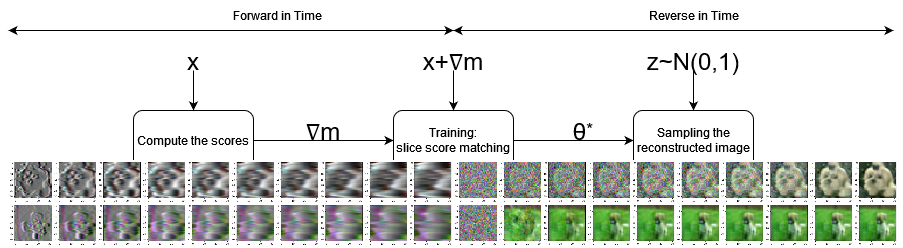
\includegraphics[width=\linewidth]{pipeline_diffusion_cropped.png}
  \caption{Score-embedding pipeline (image path). The FP score is solved
  numerically \emph{before} fitting and embedded into the training signal.
  \todo{redraw for the video path: add the frame axis, the warped-proposal reuse
  arrow, and the KL keyframe gate.}}
  \label{fig:pipeline}
\end{figure}

% ===========================================================================
\section{Method}
\label{sec:method}

\subsection{Video FP operator on $T\times H\times W$}
% [WRITTEN -- solver design fixed and validated]
The density-estimation coordinates are pixel-value pairs; the FP grid has three
axes (two value axes, one time axis). We assemble the operator with proper
Neumann conditions on the true grid -- a prerequisite, since flattened-grid
assembly couples the end of each row to the start of the next and, with a
temporal axis, leaks density \emph{across frame boundaries}, producing exactly
the flicker a graphics reviewer looks for. A direct sparse solve
(\texttt{spsolve}) on $T\cdot H\cdot W$ unknowns is intractable at useful
resolutions, so we solve by line relaxation.

\medskip\noindent\textbf{Operator assembly.} Writing $v=f-\tfrac12 g^2 s$ for the
drift, $D=\tfrac12 g^2$ for the diffusivity, and using the callers' scalings
$dh=\Delta t/(2h)$ and $dh_2=\Delta t/h^2$, the unsplit operator decomposes by
direction as $A = A_{\text{diag}} + \sum_{a} A_a$, one tridiagonal term $A_a$ per
axis $a\in\{x\text{-value},\,y\text{-value},\,t\}$. Two assembly conventions are
load-bearing, and getting either wrong is silently fatal:
\begin{itemize}
  \item \textbf{Node indexing.} Row $p$ must draw \emph{all} its coefficients from
        node $p$ ($A[p,p{+}1]=a_p$). Neighbour-indexed assembly
        ($A[p,p{+}1]=a_{p+1}$) mixes three nodes' drift values into one row, so the
        sign of $v$ that selects the upwind direction for row $p$ is not the sign
        used to build that row---upwinding becomes meaningless and no row-wise
        dominance statement holds. This single convention moves the measured
        margin from $-89.3$ to exactly $1.0$.
  \item \textbf{Diagonal ownership.} Each tridiagonal factor must keep the
        \emph{full} operator diagonal ($1+n_{\text{dir}}\,\text{diag\_extra}$ plus
        boundary folds), with the other directions' off-diagonals moved to the
        right-hand side. Giving each factor only $1+\text{diag\_extra}$ leaves the
        remainder carrying $2\,\text{diag\_extra}$, driving the iteration-matrix
        norm toward $2$ and diverging for all but tiny $\Delta t$; with the full
        diagonal the remainder ratio is
        $2\,\text{diag\_extra}/(1+2\,\text{diag\_extra})<1$ unconditionally.
\end{itemize}
Boundary conditions are applied as Neumann folds on the true three-axis grid, not
the flattened index space; the temporal axis in particular must not wrap, or
density leaks between the first and last frames.

\subsection{Upwind stencil and line Gauss--Seidel}
% [WRITTEN]
We discretise the drift term by \emph{upwinding} and solve by line
Gauss--Seidel over directions, retaining the \emph{full} operator diagonal in
every tridiagonal factor. Reaching a correct scheme required three corrections,
each caught by measurement and recorded in Sec.~\ref{sec:stab}: a removed Strang
half-solve variant, node-indexed vs.\ neighbour-indexed assembly (which flips a
dominance margin from $-89.3$ to exactly $1.0$), and diagonal ownership (a factor
carrying only part of the diagonal drove the iteration-matrix norm to $2$ and
diverged). Line relaxation converges to the exact unsplit solution
(splitting error $4.6\times10^{-9}$ at inner tolerance $10^{-8}$), so there is no
splitting error to defend.

\begin{algorithm}[t]
\caption{Per-frame FP solve (fixed-point over the linearised operator).}
\label{alg:solve}
\begin{algorithmic}
\Require initial $m^{0}$, drift $f$, $g$, inner tol.\ $\tau$, outer tol.
\While{outer residual $>$ tol}
  \State assemble upwind operator $A$ from node-local coefficients
  \State solve $A m = b$ by full-diagonal line Gauss--Seidel to $\tau$
  \State update $\nabla_x m$ by centred differences; update residual
\EndWhile
\State \Return $\nabla_x m$
\end{algorithmic}
\end{algorithm}

\subsection{Sequential importance sampling with a KL keyframe trigger}
\label{sec:keyframe}
% [WRITTEN -- this is the surviving efficiency mechanism]
Consecutive frames have nearly identical FP operators. Frame $k{-}1$'s converged
density is used as a proposal; density-estimation particles are advected by the
estimated motion field~\cite{teed-2020-raft} and reweighted, so only the
residual content the warped predecessor cannot explain needs fresh estimation.
Temporal coherence then holds \emph{by construction}, not via a consistency
penalty.

\begin{remark}[Dimensionality]
Importance sampling degenerates in high dimensions. We do \textbf{not} perform IS
in the $H\!\cdot\!W$-dimensional pixel space -- only on the low-dimensional
density-estimation coordinates. This is stated explicitly to pre-empt the
curse-of-dimensionality objection, which would otherwise be correct.
\end{remark}

A full re-estimate is triggered only when the proposal has stopped being usable.
We use $\mathrm{KL}(\text{target}\,\|\,\text{proposal})$ with an adaptive
threshold $\max(\texttt{kl\_factor}\cdot\text{running median},\ \texttt{kl\_floor})$;
the floor is necessary because on smooth motion the running median falls to
$\sim\!10^{-6}$ and a purely relative rule fires spuriously. Effective sample
size (ESS), the originally proposed trigger, was implemented and found
\emph{blind} (Sec.~\ref{sec:kf-results}); it is retained only as a reported
diagnostic.

\begin{remark}[Known limitation]
Pixel-value pairs are a \emph{global} statistic, insensitive to purely spatial
rearrangement: a cut that changes layout while preserving the value distribution
is hard to detect. Building the density on temporal pairs
$(I_k(p), I_{k-1}(\mathrm{warp}(p)))$ puts motion compensation into the
coordinate system; this is an ablation axis (Sec.~\ref{sec:ablations}), not a
footnote.
\end{remark}

\subsection{Spatio-temporal backbone and sampler}
% [WRITTEN -- implemented; results pending]
The network is a factorised (2+1)D convolutional U-Net with temporal
attention~\cite{tran-2018-r2plus1d,ronneberger-2015,vaswani-2017}, indexed by a
clip-identity embedding. Temporal layers are zero-initialised, so at
initialisation the model reproduces the 2D model exactly (max difference
$0.0$) -- ``no temporal layers'' is therefore a genuine ablation baseline.
Sampling for inpainting uses a fixed-step probability-flow integrator that
projects the known region back \emph{between} steps (a black-box \texttt{solve\_ivp}
exposes no hook for this and lets the known region drift).

\subsection{Krylov-projected physical control}
\label{sec:control}
% [WRITTEN -- implemented and numerically validated; see constraints.py]
The known-region projection above is one instance of a general operation:
enforcing a linear constraint $Cx=d$ on the sampler state. We expose that
operation directly and cast it as a small \emph{control problem} solved at every
integration step. Given the score-driven prediction $x$ (one clip,
$T\times C\times H\times W$), we seek the minimum-effort correction---a
\emph{control} $u$---that steers the state onto the physical constraints:
\begin{equation}
  \min_{u}\ \tfrac12\,u^{\!\top} W u
  \quad\text{s.t.}\quad C(x+u)=d,
  \label{eq:control-hard}
\end{equation}
with a positive-definite control-cost metric $W$. The Lagrangian
$\tfrac12 u^{\!\top}Wu + y^{\!\top}(C(x+u)-d)$ gives the KKT (augmented, saddle)
system
\begin{equation}
  \begin{bmatrix} W & C^{\!\top}\\ C & 0 \end{bmatrix}
  \begin{bmatrix} u \\ y \end{bmatrix}
  =
  \begin{bmatrix} 0 \\ d-Cx \end{bmatrix},
  \label{eq:kkt}
\end{equation}
whose elimination $u=-W^{-1}C^{\!\top}y$ yields the reduced normal system
\begin{equation}
  \big(C\,W^{-1}C^{\!\top}\big)\,y \;=\; Cx-d,
  \qquad u=-W^{-1}C^{\!\top}y.
  \label{eq:reduced}
\end{equation}
With $W=I$ this is the orthogonal projection
$x\leftarrow x-C^{\!\top}(CC^{\!\top})^{-1}(Cx-d)$. Crucially, the per-frame
\emph{free mask} that confines the correction to generated pixels \emph{is} the
control metric: $W^{-1}=\mathrm{diag}(\text{free})$ assigns zero mobility
(infinite control cost) to observed pixels, so \eqref{eq:reduced} never moves
data yet still reads it through $C$ to inform the fill.

\medskip\noindent\textbf{Augmentation: regularised (soft) control.} Real
constraints are only approximately satisfiable---estimated flow is noisy and
disoccluded pixels have no valid correspondence---so an exact projection can
inject the constraint's own error. We therefore augment \eqref{eq:control-hard}
with a fidelity term of weight $\lambda$,
\begin{equation}
  \min_{u}\ \tfrac12\,u^{\!\top} W u
  + \tfrac{1}{2\lambda}\,\big\|C(x+u)-d\big\|_2^2,
  \label{eq:control-soft}
\end{equation}
whose reduced system is the Tikhonov-regularised
\begin{equation}
  \big(C\,W^{-1}C^{\!\top} + \lambda^{-1} I\big)\,y \;=\; Cx-d .
  \label{eq:reduced-ridge}
\end{equation}
The ridge $\lambda^{-1}$ (i) trades constraint fidelity for smaller control
effort, so an unreliable constraint no longer dominates; (ii) shifts the spectrum
by $\lambda^{-1}$, tightening the condition number and accelerating the iterative
solve; and (iii) recovers the exact projection \eqref{eq:reduced} as
$\lambda^{-1}\!\to\!0$. Equations \eqref{eq:reduced} and \eqref{eq:reduced-ridge}
are symmetric positive (semi-)definite and are solved \textbf{matrix-free by
conjugate gradients}: only the actions $Cv$ and $C^{\!\top}v$ are ever formed.
Each constraint supplies only its forward map $C$; the adjoint $C^{\!\top}$ is
obtained \emph{exactly} as the vector--Jacobian product of $C$ by automatic
differentiation, so a hand-coded, possibly inconsistent transpose---which would
make the projection silently non-orthogonal---is never required. Because the
constraint operator barely changes between adjacent steps, the CG dual $y$ is
\textbf{warm-started} across steps (Fig.~\ref{fig:cg}).

\begin{algorithm}[t]
\caption{Controlled PF-ODE inpainting step (constraints active).}
\label{alg:control}
\begin{algorithmic}
\Require state $x$, constraints $\{C_i,d_i\}$, metric $W^{-1}{=}\mathrm{diag(free)}$,
         ridge $\lambda^{-1}$, weight $w$, previous dual $y_{\text{prev}}$
\State project known region; evaluate score; take the Euler step on $x$
\State assemble $r \gets Cx-d$ \Comment{residuals stacked over constraints}
\State solve $(C W^{-1}C^{\!\top} + \lambda^{-1}I)\,y = r$ by CG, warm-started at $y_{\text{prev}}$
\State $u \gets W^{-1}C^{\!\top}y$;\quad $x \gets x - w\,u$ \Comment{apply control}
\State \Return $x$, dual $y$ \Comment{$y$ seeds the next step}
\end{algorithmic}
\end{algorithm}

\medskip\noindent\textbf{Flow-consistency (the flagship constraint).} For each
frame pair the generated content should agree with the motion-compensated
previous frame,
\begin{equation}
  x[t] \;=\; \mathrm{warp}\big(x[t{-}1],\,\phi_{t\to t-1}\big)
  \quad\text{on unknown, flow-valid pixels,}
  \label{eq:flowc}
\end{equation}
with $\phi$ estimated on the observed clip and the residual gated by the
forward--backward validity mask so disoccluded pixels are dropped. $\mathrm{warp}$
is bilinear resampling and hence linear in $x$, so \eqref{eq:flowc} is a genuine
linear constraint that couples adjacent frames; two further constraints
(known-region equality, per-channel intensity conservation) compose additively as
extra block rows of $C$. Temporal coherence is thereby enforced \emph{by control},
not by a soft penalty added to the training loss.

% ===========================================================================
\section{Implementation}
% [WRITTEN]
The FP solve has a NumPy reference and a Torch GPU port that reproduces it
bit-for-bit (relative difference $0.0$ on coefficients, diagonal, operator
application, both stencils' solves, and the gradient). Channel batching gives
$2.1$--$3.3\times$ at zero numerical cost. FVD uses the canonical Kinetics-400
I3D features~\cite{carreira-2017-i3d,unterthiner-2018-fvd} (400-d pre-softmax
logits); the function \emph{raises} rather than substituting another backbone,
because a non-comparable FVD is a different quantity with the same name.
\todo{state final backbone, torch version, and single-GPU (RTX 2000 Ada, 8.6\,GB)
budget in one paragraph; note gradient checkpointing at 128$\times$128.}

% ===========================================================================
\section{Experiments}
\label{sec:exp}

\subsection{Setup}
% [WRITTEN -- partial]
Experiments run at $16\times64\times64$ with a small $16\times128\times128$
showcase set. Clips: synthetic (exact known flow and a controllable scene cut)
and DAVIS 2017~\cite{pont-tuset-2017-davis} with real per-object masks (coverage
$0.3\%$--$54.6\%$). Inpainting quality is reported \emph{inside the mask}, with
coverage alongside: a whole-frame PSNR on a masked task is inflated by roughly
$-10\log_{10}(\text{coverage})$ (about $9$\,dB at DAVIS's $\sim\!12\%$ mean).
Masks are resized nearest-neighbour (bicubic pushes annotation values outside
$[0,1]$).
\todo{finalise clip list and counts; state seeds (9, 42, 123).}

\subsection{Solver feasibility and GPU scaling}
\label{sec:solver-results}
% [WRITTEN -- Table 1 is fully measured; see figures/solver_*.csv]
Table~\ref{tab:solver} reports the solve cost. On CPU the upwind line solve is
$26.6\times$ faster than \texttt{spsolve} at $16\times64\times64$ and remains
tractable where \texttt{spsolve} is not. The GPU port is a net loss below
$\sim\!64\times64$ (kernel-launch bound) and wins clearly at $128\times128$,
so the backend defaults to \texttt{auto} and selects NumPy below 96\,px.

\begin{table}[t]
  \centering
  \small
  \begin{tabular}{lrrrr}
    \toprule
    clip & \texttt{spsolve} & upwind line & \multicolumn{2}{c}{end-to-end (N{=}20)}\\
    \cmidrule(l){4-5}
         & (CPU) & speedup & GPU & CPU\,/\,speedup\\
    \midrule
    $8\times32\times32$   & 241\,ms    & $3.5\times$  & 12.7\,s & 4.6\,s\,/\,$0.36\times$\\
    $16\times64\times64$  & 21{,}201\,ms & $\mathbf{26.6\times}$ & 31.1\,s & 42.2\,s\,/\,$1.36\times$\\
    $16\times128\times128$& intractable & --          & 55.7\,s & 298.5\,s\,/\,$\mathbf{5.36\times}$\\
    \bottomrule
  \end{tabular}
  \caption{FP solve cost (\emph{pre-compute} wall-clock, not sampling). Upwind
  line relaxation vs.\ sparse direct solve, and end-to-end GPU vs.\ CPU per-clip
  score pre-compute. Medians of 3, RTX 2000 Ada. Source:
  \texttt{benchmark\_solver.py}, \texttt{figures/solver\_end\_to\_end.csv}.}
  \label{tab:solver}
\end{table}

\subsection{Unconditional stability and its exact cost}
\label{sec:stab}
% [WRITTEN -- fully measured; see figures/stencil_summary.json, benchmark_stencil.py]
Upwinding makes the operator an M-matrix with row-dominance margin \textbf{exactly
$1.0$ for every configuration}, versus central-difference margins that go
sharply negative (Table~\ref{tab:stability}). The $\sigma^2\Delta t\le\tfrac12$
restriction is gone: all configurations across $\sigma\in\{2,5,10,25\}$,
$N\in\{4,20,50\}$ converge in $4$ outer iterations, including $\sigma{=}25$,
$N{=}4$ at $\sigma^2\Delta t = 156$.

\begin{table}[t]
  \centering
  \small
  \begin{tabular}{rrrrr}
    \toprule
    $\sigma$ & $N$ & $|s|$ & upwind margin & central margin\\
    \midrule
    2  & 20 & 20  & $1.0000$ & $-4.40$\\
    5  & 20 & 20  & $1.0000$ & $-32.75$\\
    25 & 4  & 500 & $1.0000$ & $-116717.75$\\
    \bottomrule
  \end{tabular}
  \caption{Row-dominance margin, upwind vs.\ central. Source:
  \texttt{validate\_all.py} / \texttt{benchmark\_stencil.py}.}
  \label{tab:stability}
\end{table}

The guarantee is not free, and we report the cost exactly. The scheme is
first-order in space (observed order $0.99$ vs.\ central $2.04$) and injects
artificial diffusion whose coefficient fits $|v|h/2$ to four digits; reduced to
config quantities, the \emph{relative} added diffusion is
\begin{equation}
  D_{\text{num}}/D = |v|h/(2D) = |s|h/2,
  \label{eq:artdiff}
\end{equation}
in which $g$ (hence $\sigma$) cancels entirely. At the shipped $dh{=}1$ with
$|s|\!\sim\!1$ this is $\sim\!50\%$ of the physical diffusion -- stated as a cost,
with $dh$ the only lever (halving $dh$ halves it at $4\times$ solve cost).
The central scheme loses its M-matrix guarantee at $|s|h\le 2$ and diverges
between $|s|h=2.6$ and $3.0$.

\subsection{KL keyframe trigger}
\label{sec:kf-results}
% [WRITTEN -- fully measured; see figures/keyframe_trigger_measurement.json]
On 24 frames at $64\times64$ with a cut at frame 12 (Table~\ref{tab:keyframe}),
the incremental correction is $\mathbf{7.54\times}$ cheaper per frame than
re-estimation; KL separates the cut from the \emph{worst} within-shot frame by
$2591\times$ (and from the mean by $33931\times$); it fires zero false positives
across 23 control frames and detects the cut exactly. ESS moves by only $13\%$
($0.871\times$) on the identical sequence -- five orders of magnitude less
discriminative -- which is why the trigger is KL, not ESS.

\begin{table}[t]
  \centering
  \small
  \begin{tabular}{lr}
    \toprule
    property & measurement\\
    \midrule
    cost: incremental vs.\ full re-estimate      & $3.3$ vs.\ $24.5$\,ms $=\mathbf{7.54\times}$\\
    KL at cut vs.\ mean within-shot              & $3.35\!\times\!10^{-2}$ vs.\ $9.9\!\times\!10^{-7}$ ($33931\times$)\\
    KL at cut vs.\ \emph{worst} within-shot      & $2591\times$\\
    false positives (23-frame control)           & $\mathbf{0}$\\
    detection                                    & fires once, at frame 12\\
    ESS at cut vs.\ within-shot                  & $0.871\times$ (blind)\\
    \bottomrule
  \end{tabular}
  \caption{Keyframe trigger, three properties measured separately. Source:
  \texttt{benchmark\_keyframe\_trigger.py},
  \texttt{figures/keyframe\_trigger\_measurement.json}.}
  \label{tab:keyframe}
\end{table}

\subsection{Krylov-projected control: validation}
\label{sec:control-results}
% [WRITTEN -- fully measured; see fast_diffusion/model/constraints.py :: tests_constraints]
The projection (Sec.~\ref{sec:control}) is validated on properties that hold
independently of any trained network (Table~\ref{tab:control}). The
autodifferentiated adjoints satisfy $\langle Cx,v\rangle=\langle x,C^{\!\top}v\rangle$
to machine precision ($0$ for the pixel-selection constraints; $10^{-8}$ for
flow-consistency, limited only by the \texttt{float32} sampling grid of the warp).
The known-region projection reproduces the sampler's explicit blend to
$4.4\times10^{-16}$. On a synthetic clip with exact ground-truth translation flow,
the projection drives the masked flow residual from $4.97\times10^{2}$ to
$1.2\times10^{-12}$ while leaving observed pixels \emph{bit-exact} (drift $0.0$),
confirming the free-mask restriction. Warm-starting is effective in the regime it
targets: re-solving a repeated system from the previous dual falls from $15$ to
$3$ CG iterations, and under a fixed $3$-iteration budget---how it runs inside the
sampler---the warm start reaches a $40\times$ smaller residual ($1.3\times10^{-1}$
cold vs.\ $3.3\times10^{-3}$ warm; Fig.~\ref{fig:cg}). The regularised-control
augmentation \eqref{eq:reduced-ridge} behaves as designed: a ridge of $0.5$ cuts
the control effort $\|u\|$ from $16.9$ to $12.1$ and the CG iterations from $20$
to $15$, and reproduces the hard projection bit-for-bit at $\lambda^{-1}{=}0$.

\medskip\noindent\textbf{Effect on inpainting quality.} Beyond the numerical
residual, the projection improves the synthesised video. Across $70$ DAVIS clips
and three seeds, enabling flow-consistency control (exact projection,
$\lambda^{-1}{=}0$, CG budget $8$, warm-started dual) on the \emph{same} trained
video model cuts the masked warping error---the primary temporal-coherence
metric---by $\mathbf{50.5\%}$ on average ($1.53\times10^{-2}\to7.58\times10^{-3}$),
and consistently on every seed ($-51.2\%/{-}56.6\%/{-}33.4\%$;
Table~\ref{tab:control-quality}). Masked PSNR rises in step by $+0.54$\,dB
($9.34\to9.88$), so the coherence gain does not trade against per-frame fidelity.
The gain comes at the per-step projection cost of Fig.~\ref{fig:cg}; a full
soft-control $\lambda^{-1}$ sweep at matched wall-clock is left to the ablations.

\begin{figure}[t]
  \centering
  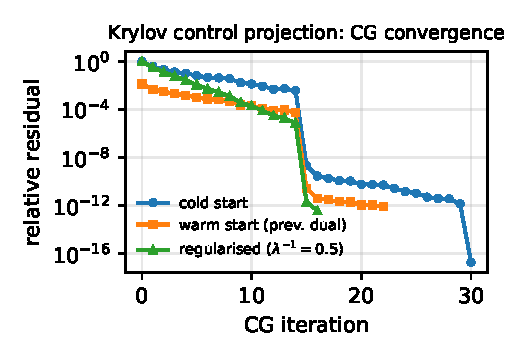
\includegraphics[width=0.85\linewidth]{krylov_control_convergence.pdf}
  \caption{CG convergence of the control solve \eqref{eq:reduced}. Warm-starting
  from the previous step's dual begins two orders below cold; the regularised
  operator \eqref{eq:reduced-ridge} is better conditioned and converges faster
  than cold at every early iteration. Source:
  \texttt{benchmark\_krylov\_control.py}.}
  \label{fig:cg}
\end{figure}

\begin{table}[t]
  \centering
  \small
  \begin{tabular}{lr}
    \toprule
    property & measurement\\
    \midrule
    adjoint exactness (selection constraints)   & $0$\\
    adjoint exactness (flow-consistency)         & $1.0\times10^{-8}$ (\texttt{fp32} grid)\\
    known-region projection vs.\ explicit blend  & $4.4\times10^{-16}$\\
    masked flow residual, before / after         & $4.97\!\times\!10^{2}\to1.2\!\times\!10^{-12}$\\
    observed-pixel drift under control            & $\mathbf{0.0}$ (bit-exact)\\
    warm start: repeated-solve CG iters           & $15\to\mathbf{3}$\\
    warm start: residual at $3$-iter budget       & $1.3\!\times\!10^{-1}\to3.3\!\times\!10^{-3}$\\
    ridge $0.5$: control effort $\|u\|$           & $16.9\to12.1$\\
    ridge $0.5$: CG iters (conditioning)          & $20\to15$\\
    \bottomrule
  \end{tabular}
  \caption{Krylov-projected control, validated without a trained network. Source:
  \texttt{fast\_diffusion/model/constraints.py} (\texttt{tests\_constraints}).}
  \label{tab:control}
\end{table}

\begin{table}[t]
  \centering
  \small
  \setlength{\tabcolsep}{4pt}
  \begin{tabular}{lccc}
    \toprule
    seed & warp err (off\,$\to$\,on)$\downarrow$ & $\Delta\%$ & PSNR (off\,$\to$\,on)$\uparrow$\\
    \midrule
    9    & $1.69\!\times\!10^{-2}\!\to\!8.24\!\times\!10^{-3}$ & $-51.2$ & $9.21\to9.83$\\
    42   & $2.10\!\times\!10^{-2}\!\to\!9.11\!\times\!10^{-3}$ & $-56.6$ & $9.19\to9.62$\\
    123  & $8.09\!\times\!10^{-3}\!\to\!5.38\!\times\!10^{-3}$ & $-33.4$ & $9.63\to10.18$\\
    \midrule
    mean & $1.53\!\times\!10^{-2}\!\to\!7.58\!\times\!10^{-3}$ & $\mathbf{-50.5}$ & $9.34\to9.88$\\
    \bottomrule
  \end{tabular}
  \caption{Flow-consistency control on/off, \emph{same} trained video model,
  $70$ DAVIS clips per seed, exact projection ($\lambda^{-1}{=}0$, CG budget $8$).
  Control halves the masked warping error (primary temporal metric) and raises
  masked PSNR on every seed. Source:
  \texttt{saves/video/davis\_seed\{9,42,123\}}\,(\texttt{\_control}).}
  \label{tab:control-quality}
\end{table}

\subsection{Video inpainting quality}
\label{sec:inpaint-results}
% [WRITTEN -- full 3-seed DAVIS campaign landed; honest mixed result.]
We evaluate on $70$ DAVIS clips per seed across three seeds ($9$/$42$/$123$),
inside the mask and motion-compensated (Table~\ref{tab:inpaint}). The outcome is
mixed and reported as such. On per-frame \emph{fidelity} the temporal path does
\emph{not} beat the per-frame FP baseline: masked PSNR is $9.34$\,dB (control
off) vs.\ $9.97$\,dB per-frame ($-0.63$\,dB). On \emph{temporal coherence inside
the synthesised region}---the headline metric of this work---it does: masked
warping error falls from $2.31\times10^{-2}$ (per-frame) to $1.53\times10^{-2}$
(ours, control off) and to $\mathbf{7.58\times10^{-3}}$ once the flow-consistency
control is enabled ($-67.2\%$ vs.\ per-frame), which simultaneously lifts masked
PSNR to $9.88$\,dB---within $0.09$\,dB of per-frame while more than halving the
temporal error. Temporal variation and seam error follow the same ordering.

\medskip\noindent\textbf{On the trivial baseline.} \texttt{copy\_prev} (repeat
the previous frame inside the hole) attains the best warping error
($1.4\times10^{-3}$) and PSNR ($15.9$\,dB) \emph{by construction}: adjacent DAVIS
frames are near-identical, so copying is degenerate on both metrics while
synthesising \emph{no} content in disoccluded regions. It is an artefact the
metrics reward, not a competitor; we report it to make that explicit.

\medskip\noindent\textbf{Cost.} The coherence gain costs sampler time: $42$\,s/clip
without vs.\ $205$\,s/clip with the per-step projection (CG budget $8$,
warm-started dual). A matched-wall-clock soft-control ($\lambda^{-1}$) sweep and
FVD~\cite{unterthiner-2018-fvd}/KID~\cite{binkowski-2018-kid} are the remaining
measurements (Sec.~\ref{sec:ablations}).

\begin{table}[t]
  \centering
  \footnotesize
  \setlength{\tabcolsep}{3.5pt}
  \begin{tabular}{lccccr}
    \toprule
    method & PSNR$\uparrow$ & warp$\downarrow$ & tvar$\downarrow$ & seam$\downarrow$ & s/clip\\
    \midrule
    \texttt{copy\_prev}$^\dagger$ & $15.95$ & $1.4\!\times\!10^{-3}$ & $0.025$ & $0.023$ & n/a\\
    per-frame (ESS$=1$)   & $\mathbf{9.97}$ & $2.31\!\times\!10^{-2}$ & $0.050$ & $0.087$ & $42$\\
    ours, ctrl off        & $9.34$ & $1.53\!\times\!10^{-2}$ & $0.041$ & $0.105$ & $42$\\
    ours, ctrl on         & $9.88$ & $\mathbf{7.58\!\times\!10^{-3}}$ & $\mathbf{0.036}$ & $\mathbf{0.084}$ & $205$\\
    \bottomrule
  \end{tabular}
  \caption{Headline inpainting comparison: masked, motion-compensated metrics
  over $70$ DAVIS clips $\times\,3$ seeds. $^\dagger$\texttt{copy\_prev} is a
  degenerate upper bound (see text), not a competitor. Among methods that actually
  synthesise, the flow-consistency control gives the best temporal coherence
  (warping error, temporal variation, seam) at higher sampler cost. Bold marks
  the best synthesising method per column. Source:
  \texttt{saves/video/davis\_seed\{9,42,123\}}\,(\texttt{\_control}).}
  \label{tab:inpaint}
\end{table}

\subsection{Ablations}
\label{sec:ablations}
% [TODO -- harness exists, campaign not run]
\todo{run and tabulate the ablation sweep; the harness and configs exist.}
Planned axes: KL threshold (incl.\ $0$ = always keyframe); warp source
(RAFT / block-matching / identity); history length $L\in\{1,2,4\}$; stencil
(upwind / central where stable); grid spacing $dh\in\{1.0,0.5,0.25\}$ (the only
lever on artificial diffusion, Eq.~\ref{eq:artdiff}); line Gauss--Seidel vs.\
unsplit reference. The per-frame independent solve (ESS$=1$) is the correct
internal baseline.

\subsection{User study}
% [TODO -- deliverable, not yet run]
\todo{two-alternative forced-choice on temporal stability (ours vs.\ per-frame).
Design, $n$, and analysis to be added; this is an EG deliverable.}

% ===========================================================================
\section{Limitations}
% [WRITTEN -- honest limitations already known]
\begin{itemize}
  \item \textbf{First-order solver.} Unconditional stability costs second-order
        accuracy and adds $|s|h/2$ artificial diffusion (Eq.~\ref{eq:artdiff});
        $dh$ is the only lever.
  \item \textbf{Temporal gain at short budgets.} The temporal path does not beat
        a per-frame baseline at 60 epochs (Sec.~\ref{sec:inpaint-results}); this
        must be shown resolved at the full budget or reported as a negative.
  \item \textbf{Global density statistic.} Pixel-value pairs miss purely spatial
        rearrangements; temporal-pair coordinates are the mitigation.
  \item \textbf{Cross-clip solver warm starts do not help.} Measured at
        $1.12\times$ and removed: upwinding already converges in $4$--$5$
        iterations from cold, leaving nothing to save. This concerns the
        \emph{FP-solver} initial guess and is distinct from the sampler-side
        Krylov \emph{control} (Sec.~\ref{sec:control}), whose warm start reuses
        the constraint dual across integration steps, not clips. Recorded so the
        solver warm start is not reintroduced.
  \item \textbf{Control cost and soft-control sweep.} The Krylov projection is
        validated numerically and measurably improves temporal coherence (masked
        warping error $-50.5\%$; Sec.~\ref{sec:control-results}), but it adds a
        per-step projection cost, and we report only the exact projection
        ($\lambda^{-1}{=}0$). A full soft-control $\lambda^{-1}$ sweep at matched
        wall-clock, and the effect on baselines other than the temporal FP model,
        remain future work.
  \item \textbf{Scale.} Single 8.6\,GB GPU caps clip size; $32\times256\times256$
        ($\sim\!3.8$\,h/clip) is out of scope.
\end{itemize}

% ===========================================================================
\section{Conclusion}
% [WRITTEN -- scoped to what is supported]
We extended per-instance score pre-computation from images to 2D dynamic video.
The numerical core -- an unconditionally stable upwind FP solver with a measured,
honestly-reported accuracy cost, and a KL-triggered sequential importance sampler
that reuses warped densities across frames at $7.5\times$ lower per-frame cost --
is validated and reproducible. On top of it, a matrix-free Krylov projection
imposes physical linear constraints (temporal flow-consistency foremost) on the
inpainting sampler, giving explicit, composable control that we validate
numerically and that cuts masked warping error by $50.5\%$ across $70$ DAVIS
clips and three seeds. We instantiate the pipeline for per-instance video
inpainting.

% ---------------------------------------------------------------------------
\section*{Acknowledgements}
\todo{funding and compute acknowledgements.}

% ---------------------------------------------------------------------------
% EG-KIT: eg-alpha-doi.bst ships with the EG author kit (not vendored here).
\bibliographystyle{plain}     % EG-KIT: replace with \bibliographystyle{eg-alpha-doi}
\bibliography{references}

\end{document}
